\title{MAGNETISMO}
%-------------------------------------------------
\begingroup
\thispagestyle{empty}
\AddToShipoutPicture*{\put(-580,0){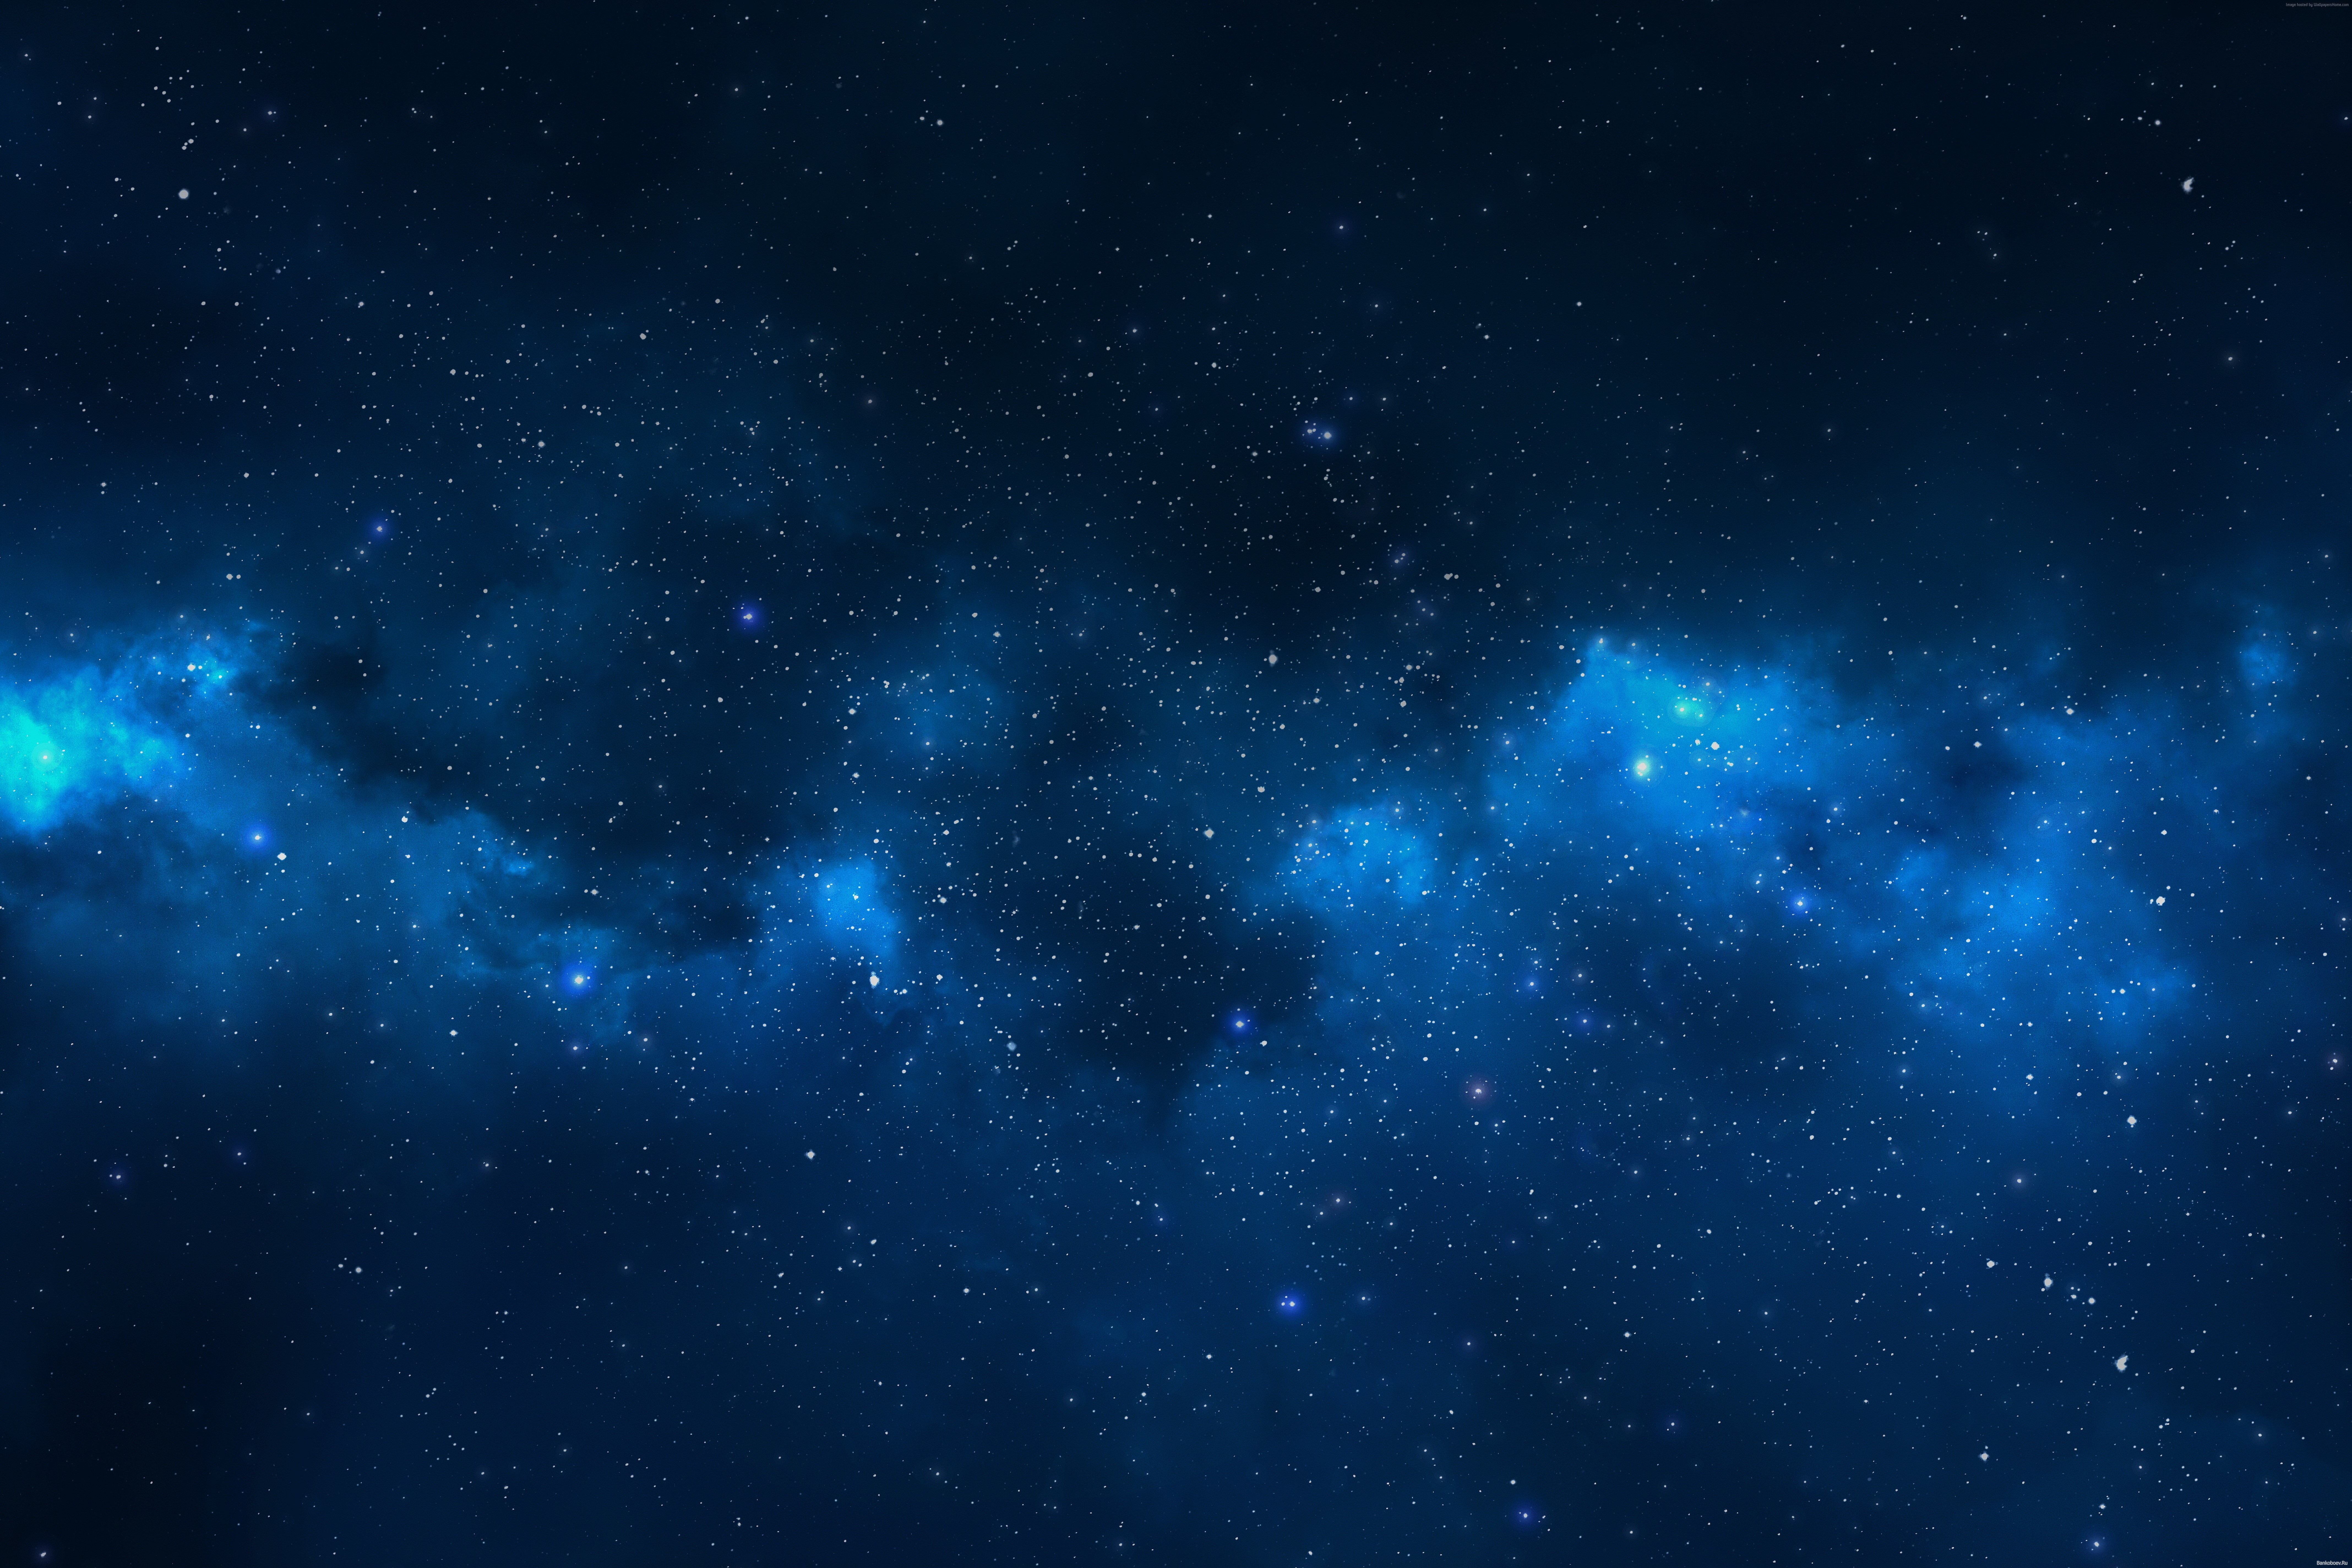
\includegraphics[scale=0.1855]{stars}}}
\centering
\vspace*{5cm}
\par\normalfont\fontsize{35}{35}\sffamily\selectfont
\textbf{Física del Magnetismo}\\
{\LARGE Notas de clase}\par
\vspace*{1cm}
%{\Huge Paolo Ricci, Ambrogio Fasoli}\par 
\endgroup
%--------------------------------------------------
\newpage
~\vfill
\thispagestyle{empty}

%\noindent Copyright \copyright\ 2014 Andrea Hidalgo\\ % Copyright notice
\noindent \textsc{Universidad Industrial de Santander \textbf{(UIS)} \\
Física Computacional en Materia Condensada  \textbf{(FICOMACO)}}\\
\url{http://www.uis.edu.co}\\

\noindent Profesor\\
Eduardo Alberto Orozco Ospino\\
eaorozco@uis.edu.co\\
\url{https://orcid.org/0000-0002-9884-9250}\\

\noindent Profesor\\
Andrés Camilo Garcia Castro\\
acgarcia@uis.edu.co\\
\url{https://orcid.org/0000-0003-3379-4495}\\

\noindent Estudiante\\
Juan Alejandro Pinto Castro\\
alejopintirris@gmail.com\\
\url{https://orcid.org/0000-0002-0937-4848}\\

\noindent \textsc{github.com/LaurethTeX/Clustering}\\ % URL

\noindent This research was done under the supervision of Dr. Pauline Barmby with the financial support of the MITACS Globalink Research Internship Award within a total of 12 weeks, from June 16th to September 5th of 2014.\\ % License information

\noindent \textit{Primera Edición, Diciembre 2018} % Printing/edition date
%--------------------------------------------------------------
\newpage
~\vfill
\thispagestyle{empty}
\noindent \begin{flushright}
\emph{"Los estudiantes que usan libros de texto de astrofísica siguen siendo esencialmente ignorantes de la propia existencia de los conceptos sobre el plasma, a pesar de que algunos de ellos se conocen desde hace medio siglo. La conclusión es que la astrofísica es demasiado importante para dejarla en manos de astrofísicos que han conseguido su conocimiento principal en estos libros de texto. Los datos de telescopios terrestres y en el espacio deben ser tratados por científicos que estén familiarizados con la física de laboratorio y de la magnetosfera, con la teoría de circuitos, y por supuesto con la moderna teoría del plasma.“\\
\vspace{3mm}
-Hannes Alfvén}
\end{flushright}

%http://www.frasesypensamientos.com.ar/autor/irving-langmuir.html
%---------------------------------------------------

\chapterimage{plasma_light_line_abstraction.jpg} % Table of contents heading image

\pagestyle{empty} % No headers
\renewcommand\contentsname{Contenido}
\tableofcontents % Print the table of contents itself

%\cleardoublepage % Forces the first chapter to start on an odd page so it's on the right

\pagestyle{fancy} % Print headers again
